\chapter{Minimum Spanning Tree in Randomized Linear Time}

\begin{problem}[MST]
Given a connected graph $G = (V, E, w)$ with distinct weights on edges, find a minimum spanning tree of $G$, i.e., a spanning tree of $G$ with the minimum total weight.
\end{problem}

To start with, we introduce a parallel algorithm on MST:

\begin{algorithm}[H]
	\caption{Boruvka's Algorithm}
	$T \gets \emptyset$\;
	$G' \gets G$\;
	\While{$G'$ is not a single vertex}{
		$A \gets \emptyset$\;
		\ForEach{vertex $v$ in $G'$ in parallel}{
			Find the minimum weight edge $e$ incident to $v$\;
			$A \gets A \cup \{e\}$\;
		}
		$T \gets T \cup A$\;
		$G' \gets G'$ after contracting all components in $A$ (discarding self-loops and keeping the lightest edge between any two components)\;
	}
	\Return $T$\;
\end{algorithm}

After $k$ Boruvka steps, the number of vertices in $G'$ is at most $\frac{n}{2^k}$. Therefore, we run at most $\log n$ Boruvka steps, and the running time for each step is linear by scanning all edges.

\section{Random Sampling}

Try sampling edges with probability $1/2$, then compute the minimum spanning forest \textcolor{blue}{$F$} of the new graph $G' = (V, E')$. Then, edges in $E'\setminus F$ are not in the minimum spanning tree of $G$, because it's the heaviest edge in some cycle.

Then we classify the edges in $E\setminus E'$ when we bring them back. Denote $e$ is \textcolor{red}{$F$-heavy} if it is the heaviest edge on the cycle in $F\cup \{e\}$, and \textcolor{blue}{$F$-light} otherwise. We can show that $F$-heavy edges are not in the minimum spanning tree of $G$, therefore one can perform MST only in $F$-light edges.

\begin{center}
	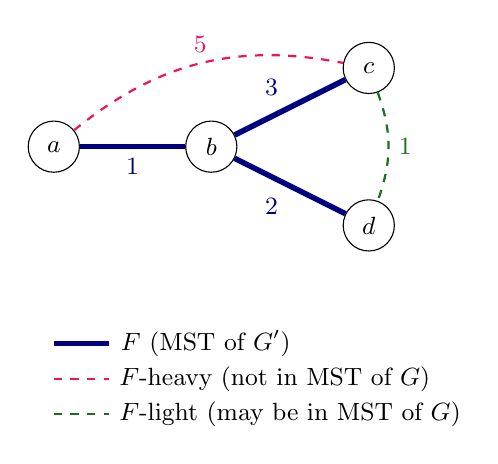
\begin{tikzpicture}[
			vertex/.style={circle, draw, fill=white, minimum size=0.65cm, inner sep=0pt, font=\small},
			tree/.style={line width=2pt, NavyBlue},
			heavy/.style={dashed, WildStrawberry, thick},
			light/.style={dashed, ForestGreen!80!black, thick},
		]
		\node[vertex] (a) at (0, 0) {$a$};
		\node[vertex] (b) at (2, 0) {$b$};
		\node[vertex] (c) at (4, 1) {$c$};
		\node[vertex] (d) at (4,-1) {$d$};

		\draw[tree]  (a) --                node[below, font=\small]      {$1$} (b);
		\draw[tree]  (b) --                node[above left, font=\small] {$3$} (c);
		\draw[tree]  (b) --                node[below left, font=\small] {$2$} (d);
		\draw[heavy] (a) to[bend left=25]  node[above, font=\small]      {$5$} (c);
		\draw[light] (c) to[bend left=20]  node[right, font=\small]      {$1$} (d);

		\begin{scope}[shift={(0, -2.5)}]
			\draw[tree]  (0, 0)    -- (0.7, 0)    node[right, font=\small, black] {$F$ (MST of $G'$)};
			\draw[heavy] (0,-0.45) -- (0.7,-0.45) node[right, font=\small, black] {$F$-heavy (not in MST of $G$)};
			\draw[light] (0,-0.9)  -- (0.7,-0.9)  node[right, font=\small, black] {$F$-light (may be in MST of $G$)};
		\end{scope}
	\end{tikzpicture}
\end{center}

\begin{theorem}
	The expectation of number of $F$-light edges is upper bounded by $2(n-1)$.
\end{theorem}
\begin{proof}
	Assume we flip a coin in the order of increasing weight of edges. If it is HEADS, we put it in $E'$, otherwise we put it in $E\setminus E'$.

	Similar to the proof of Kruskal's algorithm, we can know whether the edge is $F$-light even before we flip the coin of this edge: if adding $e$ to $F$ forms a cycle, $e$ is $F$-heavy (as it is the heaviest edge in the cycle), otherwise $e$ is $F$-light.

	Therefore, we can classify edges by flipping a penny for $F$-light edges, and flipping a nickel for $F$-heavy edges. There're 4 cases for every edge:

	\begin{itemize}
		\item Penny HEADS: $e$ is in $F$ (and in $F$-light)
		\item Penny TAILS: $e$ is in $F$-light
		\item Nickel HEADS: $e\in E'$, but not in MST
		\item Nickel TAILS: $e\not\in E'$, and not in MST
	\end{itemize}

	We know the number of $F$-light edges is the sum of Penny HEADS and Penny TAILS. In a graph, any MST has at most $n-1$ edges, so the number of Penny HEADS is at most $n-1$.

	Define $X$ as the number of penny flips until we get $n-1$ HEADS. Then $X = X_1 + X_2 + \cdots + X_{n-1}$, where $X_i$ is the number of flips until we get the $i$-th HEAD after we get the $(i-1)$-th HEAD. Each $X_i$ follows geometric distribution with parameter $1/2$, so $\E[X_i] = 2$. Therefore, $\E[X] = 2(n-1)$, which is an upper bound for the number of $F$-light edges.
\end{proof}

We have a surprising result here: the number of $F$-light edges doesn't depend on the number of edges, but on the number of vertices. Here we present the following algorithm:

\begin{algorithm}[H]
	\caption{RandMST} \label{alg:randmst}
	\If {$|V(G)| = 1$}{
		\Return $\emptyset$\;
	}
	$G_0 \gets$ the contracted graph after 2 Boruvka steps on $G$\;
	$G' \gets$ the graph after sampling edges in $G_0$ with probability $1/2$\;
	$F \gets \text{RandMST} (G')$\;
	Partition $E(G_0)$ into $F$-light edges $E'$ and $F$-heavy edges\;
	$F^* \gets \text{RandMST} (G^* = (V(G_0), E'))$\;
	\Return $F^*$ and the edges contracted in the first 2 Boruvka steps\;
\end{algorithm}

The correctness are now evident: all discarded edges are either $F$-heavy or redundant edges after Boruvka steps. According to Cycle Property in Theorem~\ref{theorem:cycle-cut}, they are not in the MST of $G$.

\section{Time Analysis}

We first assume partitioning edges takes linear time $m+n$. Denote the expected running time of this algorithm as $T(m,n)$, $G'$ has $Y$ edges, and $G^*$ has $X$ edges. Then we have the following recurrence:

\[ T(m,n) = \E[T(Y, n/4)] + E[T(X, n/4)] + m + n \]

We have $\E[Y] = m/2$ and $\E[X] \le 2(n/4 - 1) \le n/2$. Therefore, inductively, if we assume $T(m,n) \le cm+c'n$ for small $m$ and $n$, then we have
\begin{align*}
	T(m,n) & \le \E[cY + c'(n/4)] + \E[cX + c'(n/4)] + m + n \\
	       & = c'n/4 + c'n/4 + c\E[Y] + c \E[X] + m + n      \\
	       & = (c/2 + 1)m + (c/2 + c' + 1)n                  \\
	       & \le cm + c'n \quad \text{ if } c = 2, c' = 4
\end{align*}

Then it suffices to prove classifying edges takes linear time.

\section{MST Verification}

\begin{problem}[MST Verification]
Given a spanning tree $T$ and a set of non-tree edges $E$, for each $e\in E$, return whether $e$ is the heaviest edge in the unique cycle formed by adding $e$ to $T$.
\end{problem}

\begin{theorem}
	MST Verification can be solved with a linear number of comparisons.
\end{theorem}
\begin{proof}
	For the sake of simplicity, we assume $T$ is a full branching tree that:
	\begin{itemize}
		\item All leaves are at the same level
		\item All the non-tree edges go from the leaves to the ancestors
	\end{itemize}
	We omit the process of constructing such a tree from any general trees. It's worth mentioning, though, that for general non-tree edges with weight $w$, we can locate the Lowest Common Ancestor (LCA) of the two endpoints, and connect the LCA to the two endpoints with edges of weight $w$.

	\begin{center}
		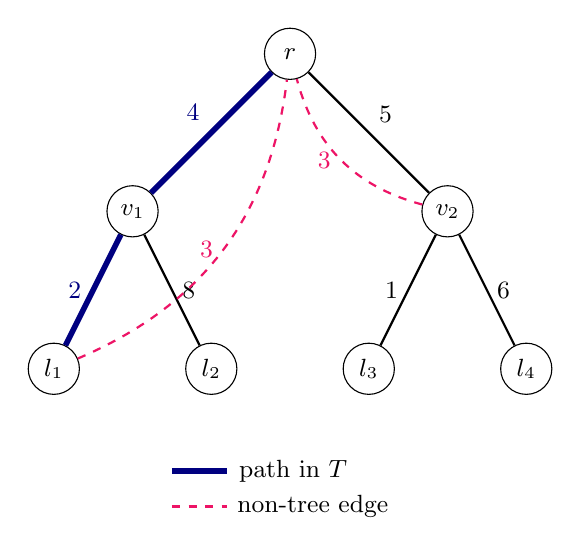
\begin{tikzpicture}[
				vertex/.style={circle, draw, fill=white, minimum size=0.65cm, inner sep=0pt, font=\small},
				tree/.style={thick},
				qpath/.style={line width=2pt, NavyBlue},
				nontree/.style={dashed, WildStrawberry, thick},
			]
			\node[vertex] (r)  at (4, 4) {$r$};
			\node[vertex] (v1) at (2, 2) {$v_1$};
			\node[vertex] (v2) at (6, 2) {$v_2$};
			\node[vertex] (l1) at (1, 0) {$l_1$};
			\node[vertex] (l2) at (3, 0) {$l_2$};
			\node[vertex] (l3) at (5, 0) {$l_3$};
			\node[vertex] (l4) at (7, 0) {$l_4$};

			% Highlighted path l1→v1→r (the max-weight query path for non-tree edge e)
			\draw[qpath] (l1) -- node[left, font=\small]       {$2$} (v1);
			\draw[qpath] (v1) -- node[above left, font=\small] {$4$} (r);
			% Other tree edges
			\draw[tree]  (r)  -- node[above right, font=\small] {$5$} (v2);
			\draw[tree]  (v1) -- node[right, font=\small]       {$8$} (l2);
			\draw[tree]  (v2) -- node[left, font=\small]        {$1$} (l3);
			\draw[tree]  (v2) -- node[right, font=\small]       {$6$} (l4);

			% Non-tree edge: leaf l1 → ancestor r
			\draw[nontree] (l1) to[bend right=30] node[left, font=\small] {$3$} (r);
			\draw[nontree] (v2) to[bend left=30] node[left, font=\small] {$3$} (r);

			% Legend
			\begin{scope}[shift={(2.5, -1.3)}]
				\draw[qpath]   (0, 0)    -- (0.7, 0)    node[right, font=\small, black] {path in $T$};
				\draw[nontree] (0,-0.45) -- (0.7,-0.45) node[right, font=\small, black] {non-tree edge};
			\end{scope}
		\end{tikzpicture}
	\end{center}

	Then the problem becomes finding the maximum weight edge on some paths from a node to its ancestors.

	Assume, for a vertex $u$, we have solved the problem from $u$ to all the ancestors $u_0, u_1, u_2, u_3, \cdots$. As the corresponding path $P_0 \subset P_1 \subset P_2 \subset P_3 \subset \cdots$, we can know the maximum length is monotonic, i.e. $\max_{e\in P_0} w(e) \le \max_{e\in P_1} w(e) \le \max_{e\in P_2} w(e) \le \cdots$.

	Then we continue on $u$'s child, $v$. $v$ has some edges to its ancestors, and for each edge, we can perform a binary search on the maximum values from this ancestor to the root. Afterward, we update the maximums that are smaller than the weight of the new edge.

	Denote $A(u)$ as the set of paths from $u$'s descendants to their ancestors.

	The number of comparisons for one binary search on $u$'s children is $O(\log(|A(u)|+1)$. Therefore,

	\[
		\text{total time} = \sum_{i \text{ as level}}^{\log n}\sum_{v\text{ in level } i} O(\log(|A(v)|+1)) \]

	One can see that $A(v) \subset A(u)$. Following this claim (we omit the rest of the proof), we have

	\[\text{total time} = O(n\log\frac{m+n}{n})) + 2m \]
\end{proof}



